
Finally, because our data has a high degree of geographic correlation, it is important to consider other time-varying factors that might be confounding the analysis. While one cannot possibly hope to exhaust all such possible confounders, we do think it appropriate to consider one obvious confounder: weather. \textcite{Gomez2007} presents regression estimates of the effect of rain and snow on turnout and propoensity to vote Repbulican. They find that for every inch of rain above the normal amount of rain a place gets, there is on average about a 0.83\% decrease in turnout and about a 2\% increase in Republican vote. Since weather is also spatially correlated, it has the potential to confound the estimates for our vote-share dependent variable (although not for our dependent variables based on donations). The perfect storm, so to speak, would be if it rained heavily along I-76 and I-95 (Southern Pennsylvania and Western New Jersey, respectively) in 2004, but nowhere else in 2004, and everywhere else in 2000. 

Fortunately, the perfect storm did not happen.  Figure \ref{fig:precipitation} presents precipitation maps from November 7th, 2000 and Nov 2nd, 2004 as reported by the National Oceanic and Atmospheric Administration (NOAA). According to these maps, on election day 2000 there was about $\nicefrac{1}{100^{\mathrm{th}}}$ an inch of precipitation in Western Pennsylvania, while on election day 2004 there was about $\nicefrac{1}{4^{\mathrm{th}}}$ of an inch of rain in Western Pennsylvania, about $\nicefrac{1}{10^{\mathrm{th}}}$ of an inch in Central Pennsylvania, and a touch of rain around New York City. This is not a great deal of rain. Historical data available through Weather Underground characterizes conditions in the apparent epicenter, Pittsburgh, as ``light rain'' for most of the afternoon, cloudy in the morning and evening, with some additional rain around 9 PM. If one accepts the estimates in \textcite{Gomez2007}, the rain differential between 2004 and 2000 is not enough to make a significant dent in our estimates, even in a worst case analysis.\footnote{The normal rainfall in Pennsylvania is about 0.1 inches, so a worst case analysis that assumes 0.3 inches of rain in every treated unit but a normal amount of rain in every control would still only explain a 0.4\% increase in Republican vote. The effect we found was an order of magnitude larger. }  Moreover, the rain appears to affect treated and control regions evenly in 2004, if anything control regions were hit harder. To be especially sure that rain has not interfered our inference, we estimate the effect on turnout due to EZ-Pass.  We find that there was no significant effect on turnout, which one would expect if rain was a serious confounder, and indeed the sign goes the opposite direction.

\begin{figure}[t]
    \centering
    \begin{subfigure}[b]{0.45\textwidth}
        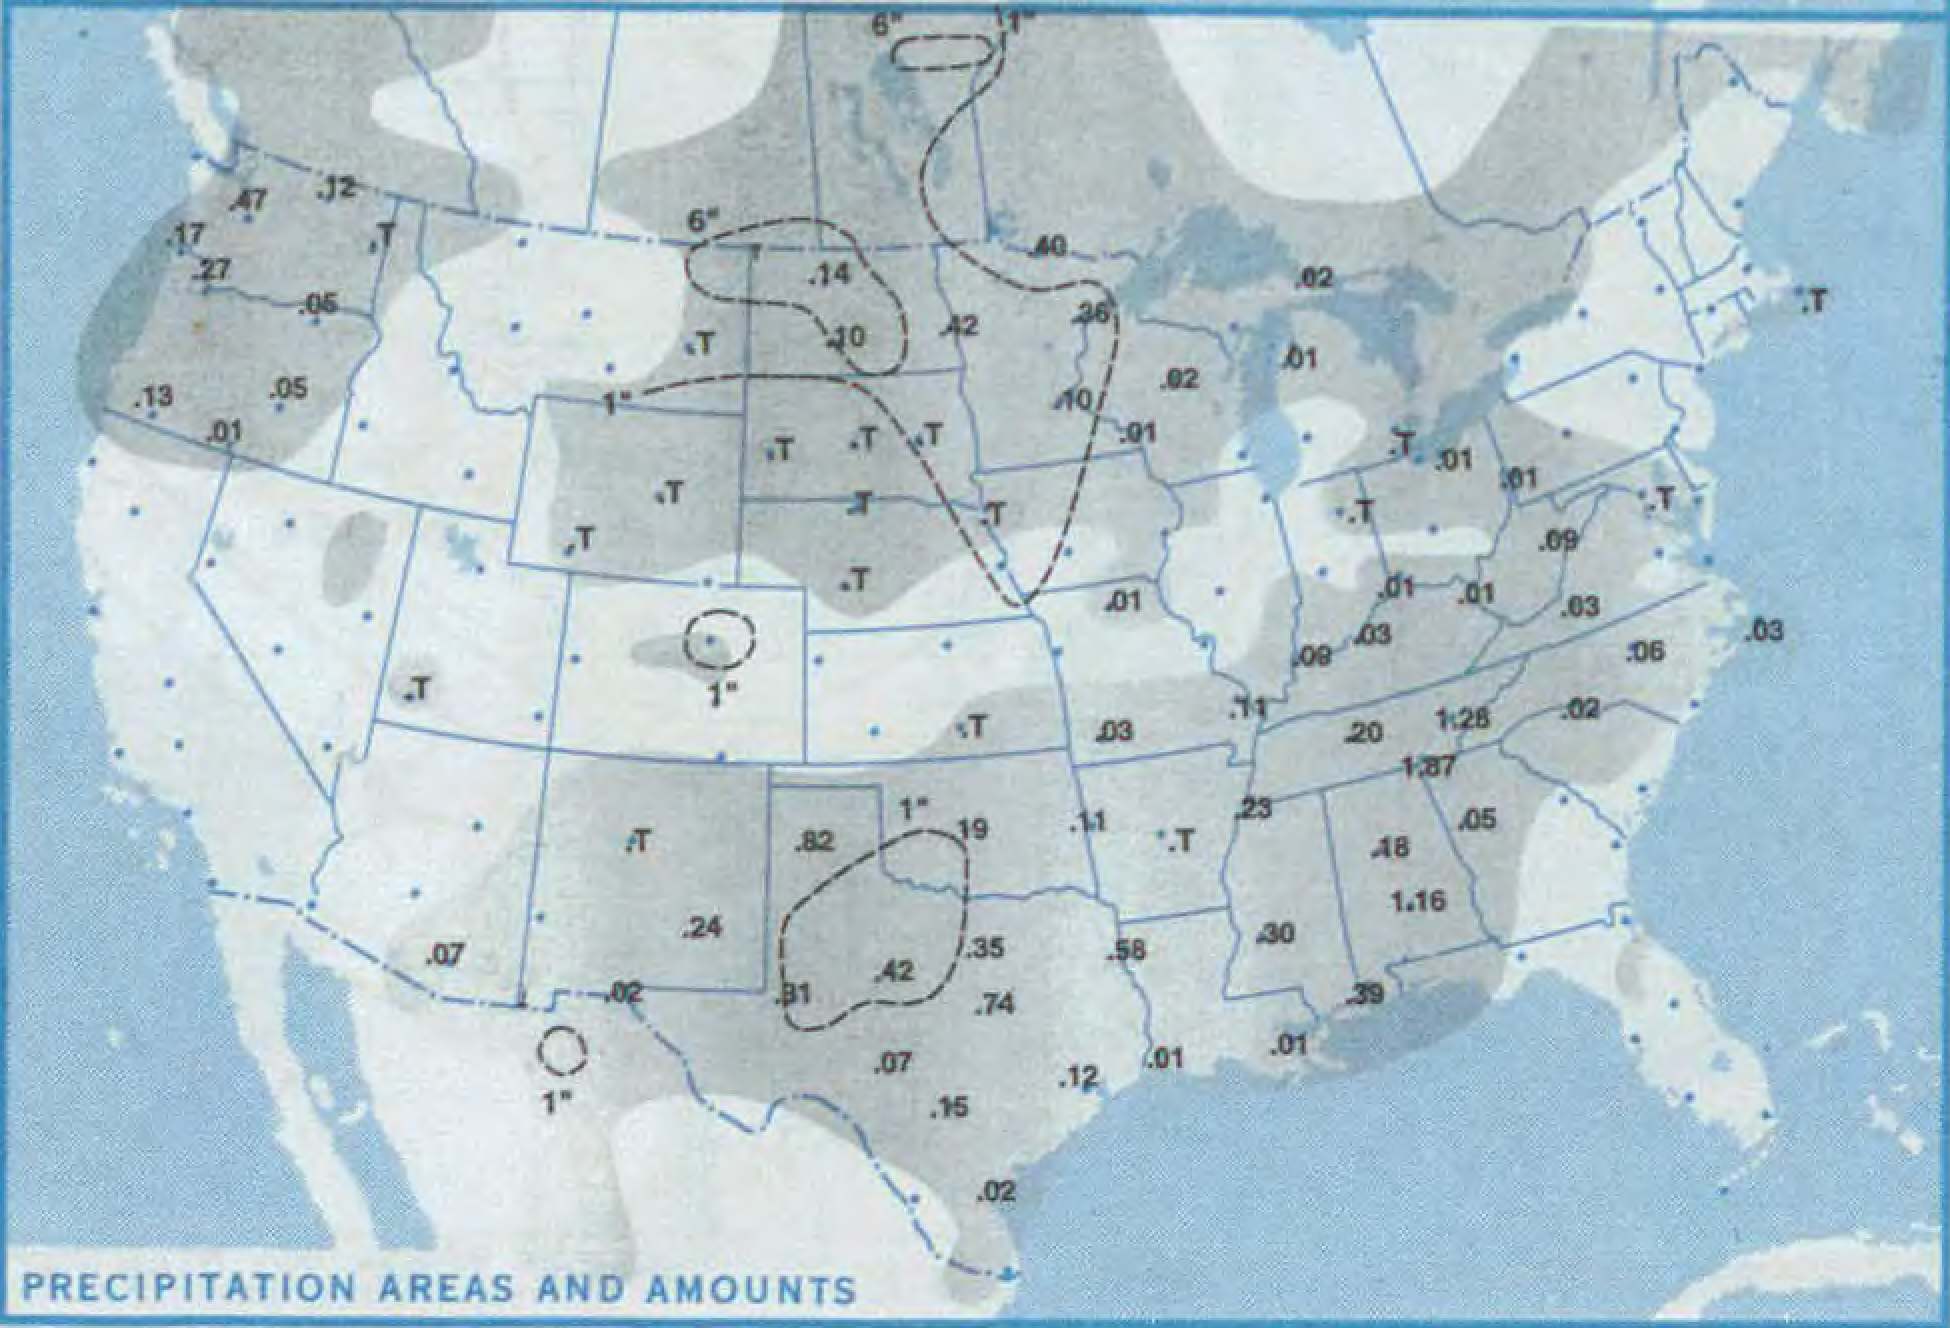
\includegraphics[width=\textwidth]{Figures/Election_2000_wednesday.png}
        \caption{7AM Nov. 7 - 7AM Nov. 8, 2000}
        \label{fig:gull}
    \end{subfigure}
    ~ %add desired spacing between images, e. g. ~, \quad, \qquad, \hfill etc. 
      %(or a blank line to force the subfigure onto a new line)
    \begin{subfigure}[b]{0.45\textwidth}
        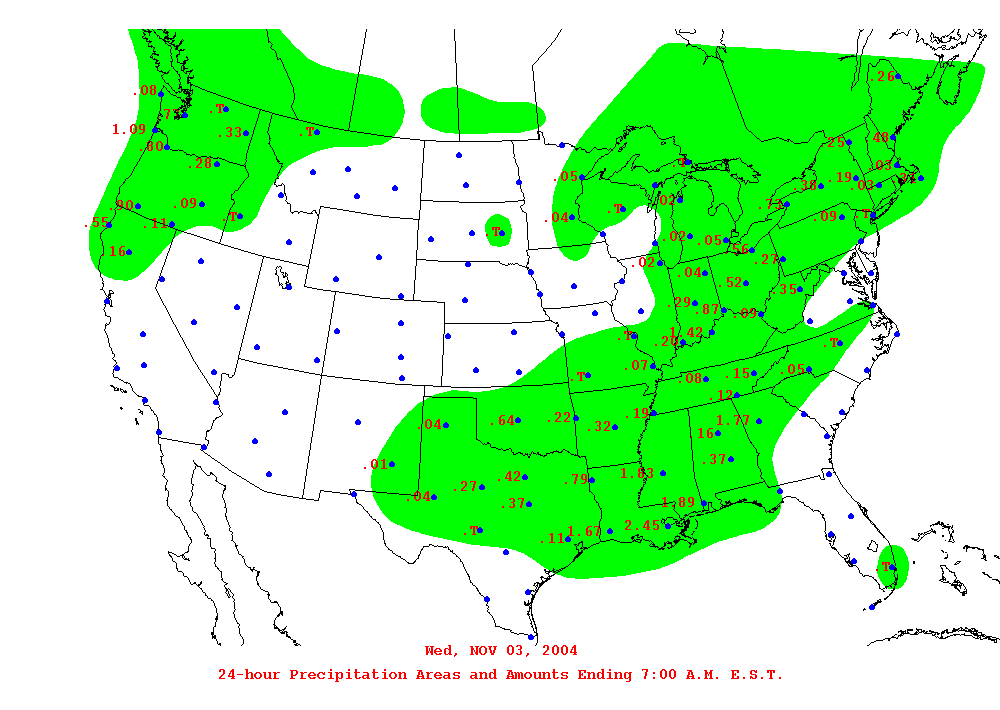
\includegraphics[width=\textwidth]{Figures/precip_20041103.png}
        \caption{7AM Nov. 2 - 7 AM Nov. 8, 2000}
        \label{fig:tiger}
    \end{subfigure}
    \caption{National weather maps from the two election days used in our study (Source: National Oceanic and Atmospheric Administration Central Library Data Imaging Project). The chart shows areas that had precipitation during the 24 hour period starting at 7 AM EST the day indicated until 7AM EST the next day. All numbers are reported in inches rounded to the nearest $\nicefrac{1}{100^{\mathrm{th}}}$, except for \textbf{.T} which refers to trace amounts of precipitation.}\label{fig:precipitation}
\end{figure}